
%(BEGIN_QUESTION)
% Copyright 2012, Tony R. Kuphaldt, released under the Creative Commons Attribution License (v 1.0)
% This means you may do almost anything with this work of mine, so long as you give me proper credit

Suppose we have a Koyo ``CLICK'' PLC connected to three process switches as shown in this illustration:

$$\includegraphics[width=15.5cm]{i02144x01.eps}$$

Determine the process conditions (i.e. temperature, level, and pressure values) given the ``live'' display of the ladder logic program shown here:

$$\includegraphics[width=15.5cm]{i02144x02.eps}$$

Also, determine the status of the lamp connected to the PLC's {\tt Y1} output.



\underbar{file i02144}
%(END_QUESTION)





%(BEGIN_ANSWER)

Temperature = below 135 $^{o}$F

\vskip 10pt

Level = above 23 inches

\vskip 10pt

Pressure = below 17 PSI

%(END_ANSWER)





%(BEGIN_NOTES)


%INDEX% PLC, relating I/O status to virtual elements 

%(END_NOTES)


